\chapter{Node Beaconing Behavior}

Since APRS is a source-routed protocol, most of the decisions as
to how often a station should send traffic and how far that traffic should
travel are allowed to be made by the originating station. 
The existing specification for the protocol hardly touches on this issue, 
while a great deal of time and energy is spent on the development forums 
bemoaning specific examples of misbehaving members of the network.
The two major parameters under the source node's control that are considered
here are the frequency of beaconing and the routing path used for each beacon.

Being a source-routed protocol does fundamentally introduce a
moral hazard in the network. For each node in the network to enjoy the
most benefit from the network, they would want to beacon as often as possible 
with the longest path allowed by the network.
It is only by mutual trust, respect, and education that this 
logic isn't universally followed and the network is not grossly oversubscribed
in the self-interest of every individual network node. 
Unfortunately, the most popular documentation on APRS fails to stress the 
importance of correctly configuring nodes in the best interest for the network
at large, and rarely gives any concrete guidance on what values should typically
be used when configuring various types of network nodes.


\section{Beaconing Algorithms}

For each APRS node with information available for the network,
a local decision needs to be made as to when that information will best 
serve the local network and should be transmitted. This is rarely a trivial 
decision, and one that could warrant much more creative and application or data
specific solutions than the ones presented here, which should be considered 
the typical minimum of most popular APRS trackers. The only datum considered 
in this work is that of a mobile node's position, but these algorithms would
likely extend to most other user applications of APRS.

\subsection{Fixed Interval Beaconing}

The simplest beaconing algorithm consists of waiting a single fixed interval
between beacons, and only requires a single parameter that is the beacon interval.
When a tracker is turned on, it acquires a GPS lock and immediately sends out a 
beacon and starts a timer. Once that timer exceeds the beacon interval value, a 
new position is acquired from the GPS receiver and the new location is beaconed.
While simple, this algorithm does suffer from a number of inadequacies:
\begin{itemize}
\item The decision to beacon is made solely based on how long it has been
since the previous beacon, without considering any other information available
to the tracker. Examples of additional information would include whether the 
tracker has moved, how fast the tracker is moving, or any packets received from
the APRS network since the last beacon.
\item A single fixed interval limits the amount of entropy introduced into the
network with regards to inter-packet arrival at other nodes. Since APRS is a 
CSMA shared channel network, it's tempting to use Poisson distribution models
for network capacity, which is likely invalid when the only source of entropy 
per tracker is the time when it was last turned on or gained GPS lock.
This is discussed further in the next chapter.
\end{itemize}

There are of course several possible extensions to the fixed interval beaconing
algorithm which each fix various deficiencies at the expense of simplicity.

\subsection{Time Slot Interval Beaconing}
\label{subsec:timeslot}

Arguably a more restrictive form of fixed interval beaconing, time slotting is 
based on the idea of preventing channel collisions by allocating each tracker
a fixed time slot in each interval for when they are allowed to transmit.
An unfeasible solution for the national APRS network due to its scale and lack
of coordination, time slotting is often applied where unusually high levels of
coordination do exist, such as special events and insular networks.

Time slotting introduces a new parameter called the slot time, and depends on every
tracker using it having synchronized real time clocks, which is reasonable since most
GPS receivers provide real time to within typically 200ms of UTC 
as part of their position reports.\footnote{The 200ms 
	uncertainty is a typical value due to the delivery of time over
an asynchronous 4800 baud serial port. Internally, GPS receivers must maintain 
their real time clocks to several orders of magnitude higher precision than this
to be even remotely useful, but this precision isn't needed for APRS time slotting.}

The slot time determines how many seconds after the beginning of each interval
a tracker should beacon. The beginning of each interval is defined by the top of
the UTC hour,\footnote{Specifying to use UTC time is remarkably 
	important, since UTC and GPS time have currently diverged by 16 seconds due to
	only UTC including leap seconds. Most, but not all, GPS receivers correctly
	compensate for this variable offset and report correct UTC time in their
GPRMC sentences.} and intervals run successively for the remainder of the hour.
For example, a tracker configured to time slot with an interval of 550 seconds and
a time slot of 12 would beacon at the following times:
\begin{tabular}{|c|c|}
	\hline
	Time & Calculated by \\ \hline
	00:00:12 & 0*550 + 12 \\ \hline
	00:09:22 & 1*550 + 12 \\ \hline
	00:18:32 & 2*550 + 12 \\ \hline
	00:27:42 & 3*550 + 12 \\ \hline
	00:36:52 & 4*550 + 12 \\ \hline
	00:46:02 & 5*550 + 12 \\ \hline
	00:55:12 & 6*550 + 12 \\ \hline
	01:00:12 & 0*550 + 12 \\ \hline
\end{tabular}

This deterministic beaconing algorithm allows carefully designed networks to 
over-subscribe network throughput well beyond the levels expected from 
the national APRS channel with its stochastic access methods. 
On an insular network separate from the national
network, it would be possible to set an aggressively short beacon interval and 
carefully space trackers such that no two beacons collide with each other. 
This would make it possible to accomplish service levels such as
every-minute position updates from several dozen tracked vehicles, 
at the expense that there is no allowance for any additional traffic 
on the RF channel, and the network would depend on manual 
assurance that every tracker is configured to use its proper time slot.

\subsection{Nice Interval Beaconing}

Nice beaconing is a behavioral extension to fixed interval beaconing 
where trackers consider whether a ``echo"
of a position beacon is heard back from any near-by digital repeaters.
Since digipeaters tend to have much higher power transmitters and better quality
antennas than mobile trackers, once a packet is successfully received by any 
digipeater, that packet is much more likely to be received by a much larger
fraction of the target audience than directly from the low-power tracker. 
Most implementations introduce a new parameter
called nice \cite[p.~38]{ot3manual}, 
which is the number of subsequent beacons to skip when a digipeater echo is heard.

\subsection{Dithered Interval Beaconing}

One of the popular traffic models used for ALOHA-based networks assumes
that traffic enters the network as a Poisson process. 
This assumption has a number of implications for the total channel capacity, 
as will be discussed in chapter \ref{chap:channelcapacity},
but an important note for tracker behavior is the fact that fixed interval
beaconing introduces no new entropy once a tracker is activated and beaconing.

\begin{figure}
	\centering
	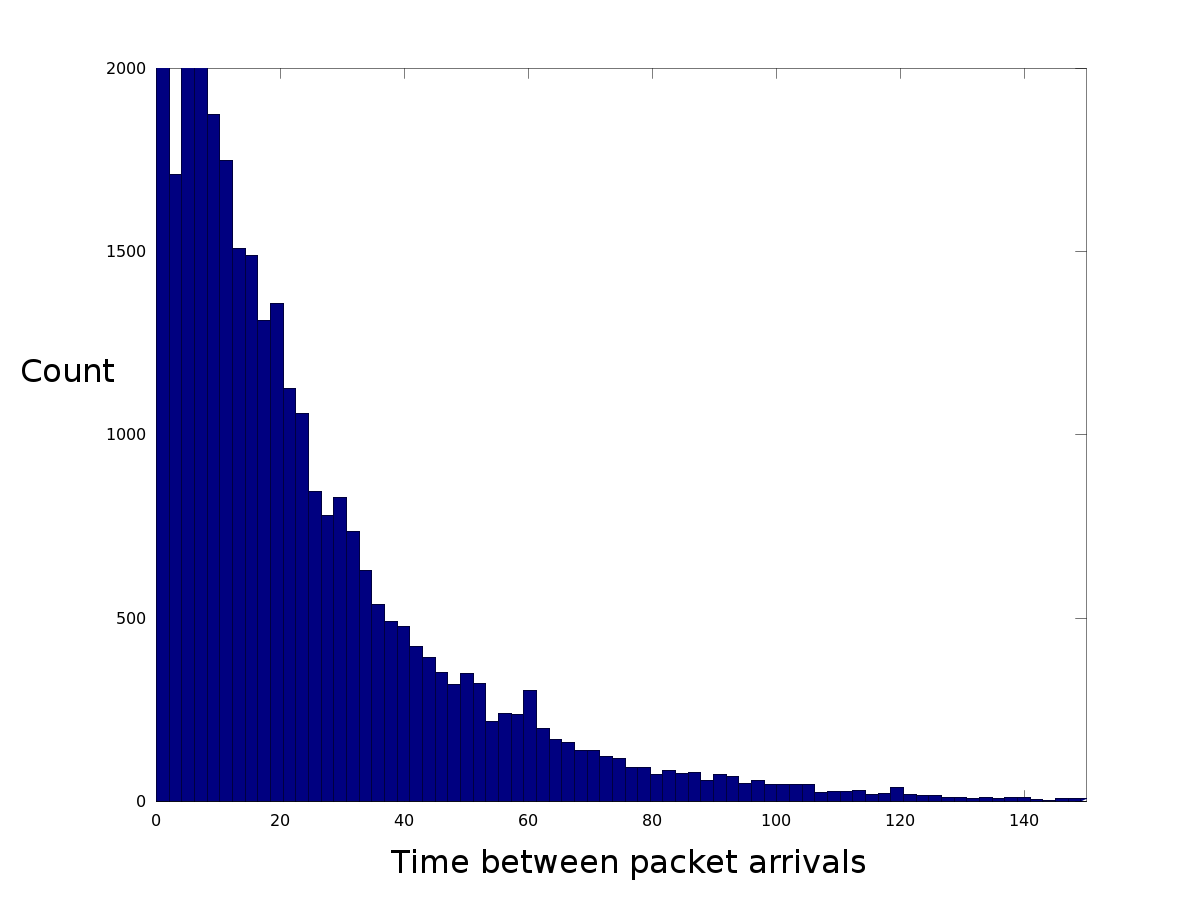
\includegraphics[width=0.7\textwidth]{src/slorfarrival}
	\caption{Packet arrival time spacing as measured over 10 days
	in San Luis Obispo, CA - TODO make better plot}
	\label{fig:rfarrivaldist}
\end{figure}

While there is no quantitative models measuring how far the current APRS 
network traffic deviates from a Poisson process, 
or how much this impacts network throughput,
observing the peaks at round numbers such as 60 and 120 second intervals
in plots such as figure \ref{fig:rfarrivaldist} indicate that the Poisson
assumption is not entirely valid.
Justifying the Poisson traffic model can be bolstered by trackers 
implementing what is called
dithering, where a small amount of noise is deliberately introduced on top
of the highly quantized beacon interval.

\begin{figure}
\begin{algorithmic}
\While {$beaconing$}
\State $interval\_delay \gets \Call{random}{ } \cdot beacon\_interval / 8$
	\State \Call{$sleep$}{$beacon\_interval + interval\_delay$}
	\State \Call{$send\_beacon$}{ }

\EndWhile
\end{algorithmic}
\caption{Beacon interval dithering algorithm}
\label{fig:ditheringalg}
\end{figure}

Developing analytic justifications for selecting specific distributions
are beyond the scope of this work, but it's theorized that introducing
any kind of entropy with approximately 1\% variance could improve network
traffic distribution.
Figure \ref{fig:ditheringalg} shows a possible implementation, where $RANDOM()$
is a function that returns a normalized distribution such as 
a uniform distribution in the range [0,1] 
or a Gaussian distribution with $\mu=0$ and $\sigma=1$.
The dividing factor of 8 was selected to scale the uniform distribution [0,1]
to yield a variance of 1\%, but that value was selected arbitrarily.

\subsection{SmartBeaconing}

SmartBeaconing\texttrademark is an adaptive beaconing algorithm developed
by Tony Arnerich and Steve Bragg for the HamHUD tracker kits \cite{smartbeacon}.
It allows trackers to make intelligent decisions as to how often to beacon
based on how ``interesting" the tracker's new position is. 
Vehicles moving in straight lines will tend to beacon at very long intervals,
but will beacon more often when making turns or traveling faster.
The algorithm is owned by HamHUD Nichetronix, LLC, and licensed freely
for non-commercial amateur radio applications.

This algorithm is particularly useful for APRS due to the fact that APRS
position reports support dead-reckoning, where they include a direction and 
velocity.
As long as trackers don't deviate from this advertised heading, there is
less reason to repeatedly beacon the tracker's new position.

The SmartBeaconing algorithm accepts up to seven parameters 
from the user\cite{smartbeaconwiki},
which are relatively more opaque than the one or two parameters required for
all the other popular interval algorithms. 
While there are suggested default values for each of these parameters, 
SmartBeaconing still proves to be controversial due to its users tending to
beacon much more often than 
trackers using other beaconing algorithms\cite{smartbeaconemail1}.
As discussed in chapter~\ref{chap:channelcapacity}, calculating the 
actual channel capacity in an area and the appropriate beaconing interval
for any of these algorithms are not at all straight forward.

\begin{table}
	\centering
	\begin{tabular}{|r|l|p{8cm}|}
		\hline
		Parameter Name & Value & Description \\ \hline
		low\_speed & 5 mph & This is the speed below which the tracker
		switches to the slow\_beacon\_interval 
		and no longer performs corner pegging. \\ \hline
		slow\_beacon\_interval & 1800 seconds & This is how often a tracker
		should beacon when it is moving slower than low\_speed, which indicates
		that it is essentially stopped. \\ \hline
		high\_speed & 60 mph & High speed is the value that slower speed
		beacon intervals are interpolated from. Speeds faster than high\_speed
		are valid but simply beacon at fast\_beacon\_interval. \\ \hline
		fast\_beacon\_interval & 180 seconds & This is how often a tracker should
		beacon when traveling at high\_speed and the scalar used to 
		calculate beacon intervals at lower speeds as a fraction of high\_speed. \\ \hline
		turn\_minimum & 30\textdegree & The absolute minimum heading change needed 
		to trigger
		a ``corner peg" where the tracker beacons sooner than its speed warrants. \\ \hline
		turn\_slope & 255\textdegree miles / hr &
		A scalar to convert between how fast a tracker is going and 
		how tight of a turn they need to perform to trigger a corner peg.
		The original documentation notes this value as unitless,
		which isn't entirely invalid since degree miles per hour isn't 
		a particularly helpful dimension. \\ \hline
		turn\_beacon\_interval & 15 seconds & The minimum time between beacons 
		when a tracker is changing heading often. \\ \hline

	\end{tabular}
	\caption{Suggested defaults for SmartBeaconing parameters}
	\label{tab:smartbeaconparams}
\end{table}

The original HamHUD algorithm is documented online as a snippet of C-like 
pseudo-code as shown in figure~\ref{fig:hamhudsmartbeacon}.
In addition to the seven algorithm parameters, the pseudo-code
requires the current speed and heading of the tracker, which are both
typically available from the \$GPRMC NMEA sentence \cite{nmearmc} provided by the 
tracker's GPS receiver, and the number of seconds since the last transmitted beacon.
Unfortunately, there are a number of issues with the provided code that
have possibly harmed deployment of the SmartBeaconing algorithm on other trackers:
\begin{itemize}
	\item Variable names change. Both ``speed" and ``mph" are used 
		to indicate the current speed of the tracker.
	\item Variable names are inconsistent. 
		slow\_rate is used for the beacon interval when the vehicle is stopped, 
		fast\_beacon\_rate for when the vehicle is moving,
		and turn\_time for when it is turning.
		A better set of variable names could be *\_beacon\_interval.
	\item The corner pegging algorithm suffers from an off-by-one error due to
		the final if statement being a $>$ comparison instead
		of a $\geq$ comparison. As documented, turning a corner would
		never cause an early beacon.
	\item The corner pegging section changes the value of secs\_since\_beacon
		instead of beacon\_rate, where secs\_since\_beacon is a system
		invariant that could possibly be implemented as a macro
		or in-line function call.
	\item The SmartBeaconing documentation specifies that 
		the velocities used are in units
		of miles per hour, where velocities expressed in the APRS
		protocol are in knots.\footnote{APRS uses knots for velocity
			due to most GPS receivers outputting location
			data as NMEA 0183 sentences, which were originally designed 
			for maritime applications.}
\end{itemize}

Due to these issues, it seemed appropriate to rewrite the algorithm 
to correct these issues and to re-typeset the pseudo-code in a more
contemporary style, which can be seen in figure~\ref{fig:kwfsmartbeacon}.

\begin{figure}[p]
\begin{lstlisting}
IF (speed < low_speed) {
	beacon_rate = slow_rate;
}
ELSE {
	// Adjust beacon rate according to speed
	IF (speed > high_speed) {
		beacon_rate = fast_beacon_rate;
	}
	ELSE {
		beacon_rate = fast_beacon_rate * high_speed / speed;
	}
	// Corner pegging - ALWAYS occurs if not "stopped"
	// Note turn threshold is speed-dependent
	turn_threshold = turn_min + turn_slope / mph;
	IF (heading_change_since_beacon > turn_threshold) AND
			(secs_since_beacon> turn_time) {
		secs_since_beacon = beacon_rate;
	}
}

IF (secs_since_beacon> beacon_rate)
	// ... send beacon
\end{lstlisting}
\caption{Original HamHUD SmartBeaconing documentation using C-like syntax}
\label{fig:hamhudsmartbeacon}
\end{figure}

\begin{figure}[p]
\begin{algorithmic}
\If {$speed < low\_speed$}
	\State $beacon\_interval\gets slow\_beacon\_interval$

	%\Comment{Clamp slow speed beacon rate and skip corner pegging}
\Else
	\If {$speed > high\_speed$}
		\State $beacon\_interval\gets fast\_beacon\_interval$    

		%\Comment{Clamp high speed beacon rate}
	\Else
		\State $beacon\_interval\gets fast\_beacon\_interval \cdot high\_speed / speed$

		%\Comment{Interpolate beacon\_rate as a fraction of fast\_beacon\_rate}
	\EndIf


	\State $turn\_threshold\gets turn\_minimum + turn\_slope / speed$
	\If {$heading\_change\_since\_beacon > turn\_threshold$}
		\State $beacon\_interval\gets turn\_beacon\_interval$

		%\Comment{Corner pegging; threshold is speed dependent}
	\EndIf
\EndIf

\If {$secs\_since\_beacon \geq beacon\_interval$}
	\State \Call{$send\_beacon$}{ }

	%\Comment{Check if enough time has elapsed to send a new beacon}
\EndIf
\end{algorithmic}
\caption{Novel presentation of SmartBeaconing algorithm by the author}
\label{fig:kwfsmartbeacon}
\end{figure}


\section{Path Recommendations}

In addition to the task of deciding when to beacon,
each user needs to make a judgment as to how far they want to flood their
traffic throughout the APRS network.
This is another subject that evokes controversy due to the problem that
recommendations that
are valid in \emph{most} of the network will often be invalid for small parts
of it.
This causes every discussion on the subject to be muddied with arguments
about small edge-cases and the specifications make no concrete recommendations
on the subject all together.

This means that the following guidance is guaranteed to be ``flawed" when
applied somewhere in the APRS network, but the hope is that this will
be generally correct when considering most of the network.
The local administrators in regions which require different path selections 
than the following should be expected to either 
maintain and publish a set of their own
recommendations or re-design their network to support the standard suggestions.

\subsection{Vehicles and Mobile Stations}

In the most general case, vehicles should use a path of ``WIDE1-1,WIDE2-1,"
which requests two total hops, including allowing low-level digis to assist
them reaching the high-level digipeater network on their first hop.
Vehicles which stay in highly populated areas should consider using the
shorter ``WIDE1-1" path, while vehicles which do the opposite and spend
a significant amount
of their time in areas with unusually sparse APRS coverage 
may use ``WIDE1-1,WIDE2-2." \cite{infoaprspath}

\subsection{Fixed Stations}

Many APRS stations aren't expected to ever move, such as home stations acting
as Internet gateways, digipeaters that are part of the infrastructure, or
remote weather stations.
Since these stations should have the transmitter power and high-quality antennas
needed to reach high-level digipeaters,
they should not begin their path with WIDE1-1 but select between the following
options depending on how many hops are needed:
\begin{itemize}
	\item WIDE2-1 - A single hop for unimportant traffic or stations near a
		particularly large coverage digipeater.
	\item WIDE2-2 - The most standard path that stations should only
		deviate from after careful consideration.
	\item WIDE3-3 - Should only be used in mountainous or spare areas for
		traffic important to a large number of stations. Very few
		stations should ever use this path.
\end{itemize}

Unlike mobile trackers,
fixed stations enjoy the advantage that they do not need to handle a
constantly changing APRS infrastructure.
Instead of using the APRS WIDE aliases, fixed stations should seriously
consider using literal paths consisting of specific digipeater callsigns.
For example, a fixed station desiring a single hop through the near-by
HIGHA digipeater should beacon with a path of ``HIGHA" instead of ``WIDE2-1."
This causes only the HIGHA digipeater to repeat the packet and not involve
any further away or lower-level digipeaters which happen to also decode the
initial transmission. 
Literal paths requesting the help of specific digipeaters is rarely
seen in APRS traffic, but should be encouraged.

Fixed stations should also consider using ``proportional pathing,"
which warrants its own section below.

\subsection{Airborne Stations}

APRS is often used as a safety or recovery system for airplanes or weather balloons,
and these stations \emph{MUST NOT} use any digipeaters in their path while
significantly above ground-level. \cite{nopathhigh}
It is critical that airborne stations use an empty path because their
altitude ensures that they already cover more area than any of the digipeaters
they would enlist to repeat their traffic.
It is common for balloons to be launched with paths such as ``WIDE1-1,WIDE2-1"
which cause havoc as packets are received by every digipeater within hundreds of
miles and needlessly repeated to other stations which have already received the
original transmission.

It may be desirable for airborne trackers to support the feature of switching from
an empty path to something else when on the ground.
A good example would be a weather balloon payload switching from an empty path
to a ``WIDE1-1" path when the balloon bursts to aid in recovery of the
payload once it reaches the ground.

\subsection{Proportional Pathing}

Proportional pathing is the tracker behavior where every beacon does not
use the same routing path, which is the norm for APRS trackers.
It is not a part of the APRS spec, but has been documented as an
errata on the aprs.org website. \cite{bobproppath}
Since information passed through the APRS network is usually more important
for stations near the originating station than those further away,
it follows that it would be preferable for near-by stations to hear these beacons
more often.
This can be accomplished by modulating the number of requested hops per beacon,
such that not every packet takes multiple hops, but some do.

A common example of where proportional pathing should be applied is
low level digipeaters.
A typical low-level digipeater beacons its location every ten minutes with
a path of ``WIDE2-1."
This means that every station within range of this digipeater, 
and every station within range of adjacent high-level digipeaters,
see the same location beacon for the unmoving digipeater every ten minutes.
It is useful to be able to see where low-level digipeaters are,
and the beacons may be required every ten minutes to meet FCC part 97 identification
requirements,
but it's unlikely that every station needs to be reassured that the digipeater
is still online every ten minutes.

Proportional pathing suggests that instead of transmitting every packet with
a path of WIDE2-1, a low-level digipeater could produce less traffic on the
APRS network by alternating between paths as follows:
\begin{table}[!h]
	\centering
	\begin{tabular}{ | r | l |}
		\hline
		Time & Path \\ \hline
		0:00 & ``~" \\ \hline
		0:10 & ``~" \\ \hline
		0:20 & ``WIDE2-1" \\ \hline
		0:30 & ``~" \\ \hline
		0:40 & ``~" \\ \hline
		0:50 & ``WIDE2-2" \\ \hline
	\end{tabular}
	\caption{Example of Proportional Pathing}
	\label{tab:exproppath}
\end{table}

At the top of the hour, 10 minutes after, 30 after, and 40 after, 
this low-level digipeater
beacons with an empty path, meaning that no other digipeaters will repeat the
packet.
Once an hour the beacon is sent requesting a single hop, and a second time
in the hour the beacon is sent with an even longer two-hop path.
This enables the digipeater to beacon every ten minutes locally,
but stations further away only have to handle its traffic once or twice an hour
while still being able to see it periodically.
The digipeater is therefore still highly visible locally, but generates
much less traffic on the high-level backbone digipeaters and further away from its
longer-range advertisements.\footnote{It's important
	to note that although the example shows every beacon at the beginning of
	every ten minutes, an actual deployment should select a random off-set
or dither their beacon interval to prevent local traffic spikes 
from happening once every ten minutes when every digi simultaneously beacons.}

This example considered the most common form of proportional pathing,
where the tracker maintains a finite state machine to switch between
a limited and predefined list of paths,
but a possible area for future work would be to develop more sophisticated
proportional pathing algorithms.
Much like the SmartBeaconing algorithm considered earlier,
heuristics could be developed to categorize how important the next beacon
will be, based on variables such as the local traffic level,
how many new stations have been recently heard, or time of day,
and used to adaptively change the routing path used.

\section{Conclusion}

This chapter has presented a list of the most popular algorithms
used to determine when a tracker should beacon, and provided some
general guidance on what routing paths should be used by different types
of trackers.
The source-routed nature of APRS is often considered a double-edge sword,
since any operator may tailor how the network
handles the local station's traffic to meet their own need.
The downside to source-routing is that malicious or ignorant stations
are empowered to cause a tremendous amount of harm to the network's performance.
There are inevitable exceptions to the guidance given in this chapter,
so modifications to any defaults should be done with careful consideration
and user education.

The guidance given has been as general as possible,
without documenting the numerous edge cases and exceptions in individual areas.
This is a common flaw with APRS documentation,
where writers refuse to give any concrete advise since it is inevitably wrong
somewhere in the world-wide APRS network.
Stations planning to operate in unusually high or low density areas should
carefully consider their beaconing behavior and consult local APRS interest
groups.\footnote{\url{http://info.aprs.net} is a particularly useful website
documenting local exceptions to these general rules.}
